\documentclass[12pt,a4paper,titlepage]{article}
\usepackage{lab_style}
\usepackage{pdfpages}
\usepackage{eso-pic}
\usepackage{graphicx}
\usepackage{float}
\newcommand\tab[1][1cm]{\hspace*{#1}}

\graphicspath{ {./} }
  
\begin{document}

\begin{titlepage}
\selectlanguage{english}

%----------------------------------------------------------------------------------------
% TITLE PAGE INFORMATION
%----------------------------------------------------------------------------------------
  \begin{center} % Center everything on the page

  %----------------------------------------------------------------------------------------
  % HEADING SECTIONS
  %----------------------------------------------------------------------------------------
  \textsc{\large Faculty of Computers, Informatics and Microelectronics}\\[0.5cm]
  \textsc{\large Technical University of Moldova}\\[1.2cm] % Name of your university/college
  \vspace{25 mm}

  \textsc{\Large Object-Oriented Modeling and Analysis}\\[0.5cm] % Major heading such as course name
  \textsc{\large Laboratory work \#4}\\[0.5cm] % Minor heading such as course title

\newcommand{\HRule}{\rule{\linewidth}{0.5mm}} % Defines a new command for the horizontal lines, change thickness here

  %----------------------------------------------------------------------------------------
  % TITLE SECTION
  %----------------------------------------------------------------------------------------
  \vspace{10 mm}
  \HRule \\[0.4cm]
  { \LARGE \bfseries Modeling your project with Collaboration Diagrams. Technologies. Design Principles. }\\[0.4cm] % Title of your document
  \HRule \\[1.5cm]

  %----------------------------------------------------------------------------------------
  % AUTHOR SECTION
  %----------------------------------------------------------------------------------------
      \vspace{30mm}

      \begin{minipage}{0.4\textwidth}
      \begin{flushleft} \large
      \emph{Author:}\\
      Cernei \textsc{Liviu}
      \end{flushleft}
      \end{minipage}
      ~
      \begin{minipage}{0.4\textwidth}
      \begin{flushright} \large
      \emph{Supervisor:} \\
      Mihail \textsc{Gavrilița} % Supervisor's Name
      \end{flushright}
      \end{minipage}\\[4cm]

      \vspace{5 mm}
      % If you don't want a supervisor, uncomment the two lines below and remove the section above
      %\Large \emph{Author:}\\
      %John \textsc{Smith}\\[3cm] % Your name

      %----------------------------------------------------------------------------------------
      % DATE SECTION
      %----------------------------------------------------------------------------------------

      {\large Chișinau 2018}\\[3cm] % Date, change the \today to a set date if you want to be precise

      %----------------------------------------------------------------------------------------
      % LOGO SECTION
      %----------------------------------------------------------------------------------------

      %\includegraphics{red}\\[0.5cm] % Include a department/university logo - this will require the graphicx package

      %----------------------------------------------------------------------------------------

      \vfill % Fill the rest of the page with whitespace
      \end{center}
      
\end{titlepage}

\cleardoublepage

\newpage

\pagenumbering{arabic}
\setcounter{page}{1}
\setcounter{secnumdepth}{4}

\addtocontents{toc}{\protect\thispagestyle{empty}} % no page number on the table of contents page
\cleardoublepage


\phantomsection
\addcontentsline{toc}{section}{Introduction}
\section*{Laboratory work \#4}
\phantomsection

\section{Tasks}
\begin{itemize}
	\item
	Model your application using 3 Collaboration Diagrams;
	\item 
	Describe the Technologies you plan on using in your project. I want to know what,
why and how you are planning to use them. Sell them to me.
\end{itemize}

\section{Theory}

\subsection{Collaboration Diagrams}
The UML Collaboration diagram is used to model how objects involved in a scenario interact, with each object instantiating a particular class in the system. Objects are connected by links, each link representing an instance of an association between the respective classes involved. The link shows messages sent between the objects, and the type of message passed (synchronous, asynchronous, simple, balking, and timeout).\par
Collaboration diagrams offer a better view of a scenario than a Sequence diagram when the modeler is trying to understand all of the effects on a given object and are therefore good for procedural design.
\clearpage

\section{Collaboration Diagrams}
In Figure ~\ref{fig:login} is represented the collaboration diagram for the login operation.
\begin{figure}[H]
	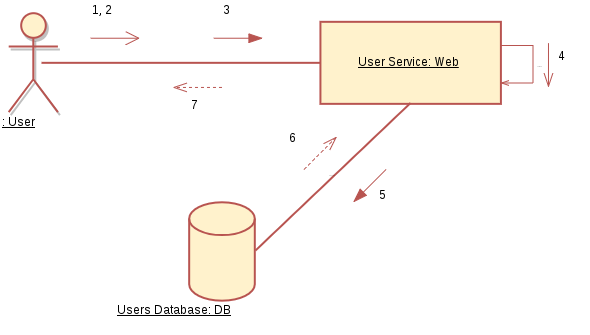
\includegraphics[width=\textwidth]{login}
	\caption{Login collaboration diagram}
	\centering
	\label{fig:login}
\end{figure}
Here we can see the interaction beween objects in our project. These diagrams are the equivalent of the previous sequence diagrams.\par
\noindent 1 - input username;
2 - input password;
3 - click login;
4 - chek input;
5 - query the user;
6 - success;
7 - authentication successful;

In Figure ~\ref{fig:create} is represented the collaboration diagram for creation of a new course.
\begin{figure}[H]
	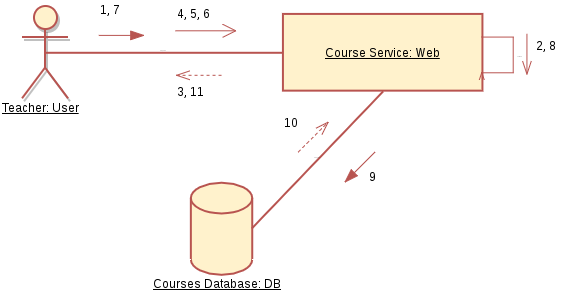
\includegraphics[width=\textwidth]{create}
	\caption{New course collaboration diagram}
	\centering
	\label{fig:create}
\end{figure}
\noindent 1 - click [New Course];
 2 - check authorization;
 3 - success;
 4 - input title;
 5 - input description;
 6 - upload content;
 7 - click [Submit];
 8 - chek input;
 9 - add new course;
10 - success;
11 - new course created;

In Figure ~\ref{fig:feedback} is represented the collaboration diagram for giving feedback for a course.
\begin{figure}[H]
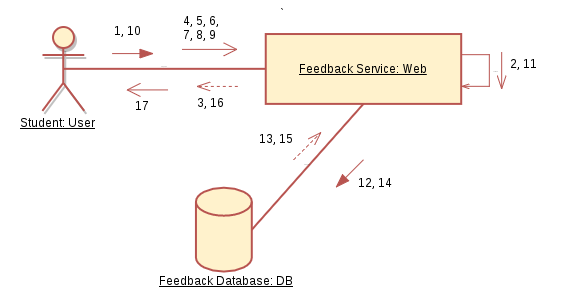
\includegraphics[width=\textwidth]{feedback}
\caption{Feedback collaboration diagram}
\centering
\label{fig:feedback}
\end{figure}
\noindent 1 - click [Give Feedback];
 2 - check if user took this course;
 3 - success;
 4 - evaluate by lectures;
 5 - evaluate by labs;
 6 - evaluate by teacher competence;
 7 - grade the course(0-10);
 8 - additional notes;
 9 - suggestions;
10 - click [Submit];
11 - chek fields;
12 - add feedback;
13 - success;
14 - calculate average mark;
15 - success;
16 - feedback submitted;
17 - average mark;

\section{MVC Pattern}
Model–view–controller is commonly used for developing software that divides an application into three interconnected parts. This is done to separate internal representations of information from the ways information is presented to and accepted from the user. The MVC design pattern decouples these major components allowing for efficient code reuse and parallel development.\par
Traditionally used for desktop graphical user interfaces (GUIs), this architecture has become popular for designing web applications and even mobile, desktop and other clients. Popular programming languages like Java, C\#, Ruby, PHP and others have popular MVC frameworks that are currently being used in web application development straight out of the box.\par
\section{Conclusion}
In this laboratory work we learned to create Collaboration Diagrams.

\clearpage
\cleardoublepage

\end{document}
